\documentclass[10pt,twocolumn,letterpaper]{article}

\usepackage{iccv}
\usepackage{times}
\usepackage{epsfig}
\usepackage{graphicx}
\usepackage{amsmath}
\usepackage{amssymb}
\usepackage{dsfont}
\usepackage{xcolor}
 \usepackage{setspace}
 
 \usepackage{caption}
 \usepackage{subcaption}
\graphicspath{ {./images/} }

\DeclareMathOperator*{\argmin}{arg\,min}
\DeclareMathOperator*{\argmax}{arg\,max}
% Include other packages here, before hyperref.

% If you comment hyperref and then uncomment it, you should delete
% egpaper.aux before re-running latex.  (Or just hit 'q' on the first latex
% run, let it finish, and you should be clear).
\usepackage[pagebackref=true,breaklinks=true,letterpaper=true,colorlinks,bookmarks=false]{hyperref}

% \iccvfinalcopy % *** Uncomment this line for the final submission

\def\iccvPaperID{623} % *** Enter the ICCV Paper ID here
\def\httilde{\mbox{\tt\raisebox{-.5ex}{\symbol{126}}}}

% Pages are numbered in submission mode, and unnumbered in camera-ready
\ificcvfinal\pagestyle{empty}\fi
\begin{document}

%%%%%%%%% TITLE
%\title{Youtube2Storyline: Unsupervised Semantic Parsing of Video Collections}
% \title{From YouTube to Semantic Storylines}
%\title{YouTube to Semantic Storylines}
\title{Unsupervised Semantic Parsing of Video Collections}
%\title{Unsupervised Grounding of Video Collections to Semantic Actions}



\author{First Author\\
Institution1\\
Institution1 address\\z
{\tt\small firstauthor@i1.org}
% For a paper whose authors are all at the same institution,
% omit the following lines up until the closing ``}''.
% Additional authors and addresses can be added with ``\and'',
% just like the second author.
% To save space, use either the email address or home page, not both
\and
Second Author\\
Institution2\\
First line of institution2 address\\
{\tt\small secondauthor@i2.org}
}

\maketitle
%\thispagestyle{empty}


%%%%%%%%% ABSTRACT
\begin{abstract}
Human communication typically has an underlying structure. This is reflected in the fact that in many user generated videos, a starting point, ending, and certain objective steps between these two can be identified. In this paper, we propose a method for parsing a video into such semantic steps in an unsupervised way. The proposed method is capable of providing a semantic ``storyline'' of the video composed of its objective steps. We accomplish this using both visual and language cues in a joint generative model. The proposed method can also provide a textual description for each of the identified semantic steps and video segments. We evaluate this method on a large number of complex YouTube videos and show results of unprecedented quality for this intricate and impactful problem.
\end{abstract}

%%%%%%%%% BODY TEXT
% !TEX root = recipeUnderstanding.tex

\section{Introduction}
Human communication takes many forms, including language and vision. For instance, explaining ``how-to'' perform a certain task can be communicated with language (e.g., Do-It-Yourself books) information as well as visual (e.g., instructional YouTube videos) information. Regardless of the form, such human-generated communication is generally structured and often has a clear beginning, end, and a set of steps in between. A typical and highly structured example is the description of an event or a procedure as the comprising steps can be clearly identified. Parsing such communication into its set of semantic steps is the key to understand human activities. With a large amount of instructional video collections, we present a method to ground and parse them into semantically meaningful actions.


%In this paper, we propose a method for decomposing a video into semantically meaningful steps in a fully unsupervised manner.

% both used.
%  With large amount of document collections, there is a huge body of work dedicated to understanding language \cite{xx,nap}.
%
% Language and vision are the two main modalities employed for this structured communication by

The two modalities of language and vision often provide different, but correlating and complementary information. Challenge lies in that both video frames and language (from sub-titles or speech recognition\footnote{Note that subtitles, generated either via Automatic Speech Recognition (ASR) or by the user, are available for most YouTube videos.}) are only a noisy, partial observations of the actions being performed. Moreover, complementary nature of language and vision, also requires us to model them jointly. In this paper, we present a unified model, learned in a fully unsupervised manner, in order to jointly use these two modalities.

% Furthermore they are
% We utilize these two modalities (video frames and imperfect automatically generated subtitles) in a unified manner in our framework;
% We qualitatively and quantitatively argue that a joint inference is crucial for a successful semantic parsing, particularly when no supervision is employed.


%  the proposed approach on instructional videos from YouTube (\eg, ``Making panckage'', ``How to tie a bow tie'') as they typically have clear steps and provide concrete grounds for demonstrating a semantically meaningful parsing. These videos are often long and manifest a high intra-class variability yet the underlying steps remains well-defined and structured, similar to almost all human communications.

The key idea in our proposed model is to capture the underlying structure in activities, while accounting for the large intra-class variability (e.g., YouTube has 281.000 videos for \emph{"How to tie a bow tie"}). We account the intra-class variation by jointly learning the entire video collection instead of a single one. We choose instructional videos (\eg, ``Making panckage'', ``How to tie a bow tie'') as they typically have clear steps and provide concrete grounds for demonstrating a semantically meaningful parsing. In principle, the proposed parsing method is applicable to any type of videos as long as they are composed of a set of steps.

The output of our method can be seen as the semantic ``storyline'' of a rather long and complex video (see Fig. \ref{fig:teaser}). This storyline provides what particular steps are taking place in the video (\emph{what}), what their semantic meaning is (\emph{how}), and when they are occurring (\emph{when}). This method is also capable of putting multiple videos performing the same overall task in common ground (i.e., the semantic steps’ space) and capture their high-level similarity, and therefore, provide a \emph{categorical} storyline as well.

In our approach, given a video, we capture the visual properties of unsupervised object proposals from each frame as well as the frequencies of keywords from the subtitle. We then employ a generative \emph{beta process mixture model}, which identifies the semantic steps shared among the videos of to the same category based on both text and visual cues. The model also identifies the text keywords which were deemed highly related to the semantic action of each steps. We later learn a language model to provide a textual description of the semantic steps based on the identified keywords.

This work is the first to provide a semantic storyline for a complex video collection. We are also the first to approach this problem in a multimodal (joint language and vision) manner. In addition, our method is capable of providing a caption describing the steps. Our approach to captioning is fundamentally different from the majority of existing video/image-to-text work in two aspects: 1) the captions are generated in an unsupervised manner, 2) our captions are \emph{descriptions} of the semantic steps, yet they are inferred from \emph{narration} of the text. This is different from the existing captioning work as their reference data is also descriptive of the visual information, while narration text often provides complementary information to the visuals and is not necessarily descriptive.

%Leaning the instructions of a novel non-trivial task is both a challenge and a necessity for both humans and autonomous systems. This necessity resulted in many community generated instruction collections \cite{wikiHow,eHow} and expert curated recipe books\cite{recipeBook1,recipeBook2}. However, this instructions are generally based on a language modality and explains a single way of performing the task although there are variety of ways. On the other hand, online video storage services are full of unstructured instructional videos\footnote{YouTube has 281.000 videos for \emph{"How to tie a bow tie"}} covering variety of ways, environment conditions and view angles. Although there have been many successful attempts in detecting activities from videos \cite{act1,act2}, structural representation of such a large and useful video collection is not possible. In this paper, we focus on joint semantic representation of YouTube videos as a response to a single query. We specifically study the unsupervised joint-detection of the activities from a collection of YouTube videos.

%Understanding of the instructional videos, requires the careful processing of two complementary modalities namely language and the vision.  Luckily the target domain, YouTube videos, has unstructured subtitles as well. They are either generated by the content developer (5\% of the time) or automatically generated by using the Automatic Speech Recognition (ASR) software. The main limitations of the existing activity detection literature for this problem is scalability and representation level. Existing approaches are mainly supervised and requires extensive training set which is not tractable in the scale of YouTube videos. Moreover, current activity detection research focuses on the low-level visual features. However, such videos in the wild have objects with completely different texture and shape characteristics from wide range of views. Instead, we focus on extracting high-level visual semantic representations and using salient words occurring among the videos.

%We rely on the assumption that the videos collected as the response of a same instructional query, share similar activities performed by the similar objects. We start with the independent processing of the videos in order to create a large collection of visual object proposals and words. After the proposal generation, we jointly process the proposal collections and words to detect the visual objects and words which can be used to represent the unstructured information. Since we rely on high-level information instead of the low-level features, the resulting objects represent the semantic information instead of visual characteristic. By using the extracted objects, we compute the holistic representation of the multi-modal information in each frame.

%Moving from frame-wise visual understanding to activity understanding, requires the joint processing of all the videos with the temporal information. In order to exploit the temporal information, we model each video as a Hidden Markov Model using state space of activities. Since we assume that the videos share some of the activities and we have no supervision, we use a model based on \emph{beta process mixture model}. Our model jointly learn the activities and detect them in the videos. Moreover, it does not require prior knowledge over the number of activities.

\section{Related Work}
Three key aspects differentiate this work from the majority of existing techniques for similar tasks: 1) capability of providing a semantic parsing of a video category leading to a compact storyline representation, 2) being unsupervised, 3) adopting a multi-modal joint vision-language model for video parsing. A thorough review of the related literature is provided below.

\paragraph{Video Summarization:}
Summarizing an input video as a sequence of key frames (static) or video clips (dynamic) is useful for both multimedia search interfaces and retrieval purposes. Early works in the area are summarized in \cite{vidAbstraction} and mostly focus on \emph{choosing keyframes} for visualization. Keyframes are also improved by using the video tags by Hong et al. \cite{beyondSearch} and using the spatio-temporal information by Gygli et al. \cite{createSum}.
%% AMIR: put a '~' instead of ' ' before \cite

%%AMIR: could be briefed 
Summarizing videos is particularly important for ego-centric videos as they are generally long in duration. There are many works which successfully segment such videos into a sequence of important shots \cite{lee2012discovering, lu2013story}; however, they mostly rely on characteristics specific to edge-centric videos, and therefore do not generalized to generic or instructional videos. For instance, Rui et al. \cite{rui2000automatically} proposed a dynamic summarization method based on the excitement of the speech of the reporter.

%http://www.sangminoh.org/Publications_files/Oh2012bmvc_videography.pdf --> learn atomic representations and do not do a segmentation
Summarization is also applied to the large image collections by recovering the temporal ordering and visual similarity of images \cite{storyGraph}, and by Gputa et al. ~\cite{gupta2009understanding} to videos in a supervised framework using annotations of actions as well as partial spatial and temporal relationships among the actions. The image collections are also used to choose important view points for video key-frame selection by Khosla et al.\cite{khosla2013large} and further extended to video clip selection by Kim et al.\cite{kim2014joint}, Potapov et al.\cite{potapov2014category}. Unlike all of these methods which mostly focus on forming a set of key frames/clips for a compact summary (which is not necessarily semantically meaningful), we provide a fresh approach to video summarization by performing it through semantic parsing on vision and language. Also, regardless of this dissimilarity, we experimentally compare our method against them.

\paragraph{Modeling Visual and Language Information:}
Learning the relationship between the visual and language data is a crucial problem due to its immense applications. Early methods \cite{matching} in this area focus on learning a common multi-modal space in order to jointly represent language and vision. They are further extended to learning higher level relations between object segments and words \cite{connecting}. Similarly, Zitnick et al.\cite{zitnick2013learning,zitnick2013bringing} used abstracted clip-arts to understand spatial relations of objects and their language correspondences. Kong et al. \cite{kong2014you} and Fidler et al. \cite{fidler2013sentence} both accomplished the task of learning spatial reasoning by only using the image captions. Relations extracted from image-caption pairs, are further used to help semantic parsing \cite{yu2013grounded} and activity recognition \cite{motwani2012improving}. Recent works also focus on automatic generation of image captions with underlying ideas ranging from finding similar images and transferring their captions \cite{ordonez2011im2text} to learning language models conditioned on the image features \cite{kiros2014multimodal,socher2014grounded,farhadi2010every}; their employed approach to learning language models is typically either based on graphical models \cite{farhadi2010every} or neural networks \cite{socher2014grounded,kiros2014multimodal,deepAlignment}.

All aforementioned methods are using supervised labels either as strong image-word pairs or weak image-caption pairs, while our method is fully unsupervised.

\paragraph{Activity/Event Recognition:}
The literature of human action recognition is broad. The closes techniques to our problem are either supervised or focus on detecting a particular (and often short) action in a weakly or unsupervised manner. Also, a large body of action recognition methods are intended for trimmed videos clips or remain limited to detecting very short atomic actions~\cite{kuehne2011hmdb, UCF101, niebles10_eccv, laptev08_cvpr, efros03_iccv, ryoo09_iccv}. Even though some promising recent works attempted action recognition in untrimmed videos ~\cite{THUMOS14, oneata2014lear, jainuniversity}, they are primarily fully supervised. 

Additionally, several method for localizing instances of actions in rather longer video sequences have been developed~\cite{duchenne09_iccv, hoai11_cvpr, laptev07_iccv, bojanowski14_eccv, pirsiavash14_cvpr}. Our work is different from those in terms of being multimodal, unsupervised, applicable to a video collection, and not limited to identifying predefined actions or the ones with short temporal spans.
%Representing actions as 2D+t tubes is a common strategy for action recognition~\cite{blank05_iccv, brendel11_iccv, ma13_iccv}. Recently, there are works that use hierarchical spatiotemporal segments to capture the multi-scale characteristics of actions \cite{brendel11_iccv, ma13_iccv}. Our representation differs in that we can discover the action-related spatiotemporal segments by joint processing the video collection from a pool of proposals. 
Also, the previous works on finding action primitives such as~\cite{niebles10_eccv, yao10b_cvpr, jain13_cvpr,lan14_eccv, lan14_vs} are primarily limited to discovering atomic sub-actions, and therefore fail to identify complex and high-level parts of a long video.

Recently, event recounting has attracted much interest and intends to identify the evidential segments for which a video belongs to a certain class~\cite{sun2014discover,das2013thousand,barbu2012video}. Event recounting is a relatively new topic and the existing methods mostly employ a supervised approach. Also, their end goal is to identify what parts of a video are highly related to an event, and not parsing the video into semantic steps. 
%This setup is similar to Hughes et al.\cite{npActivity}. However, we differ in the choices of the underlying distributions since we based our model on semantic multi-modal information.

% AMIR: flow graph sounds like 'storyline'. Consider replacing/removing it.
\paragraph{Recipe Understanding:}
Following the interest in community generated recipes in the web, there have been many attempts to automatically process recipes. Recent methods on natural language processing \cite{cookingSemantics,logicRecipe} focus on semantic parsing of language recipes in order to extract actions and the objects in the form of predicates. Tenorth et al.\cite{logicRecipe} further process the predicates in order to form a complete logic plan. Mori et al.\cite{flowGraph} also learns the relations of the actions in terms of a flow graph with the help of a supervision. The aforementioned approaches focus only on the language modality and they are not applicable to the videos. The recent advances \cite{beetz,cookie} in robotics use the parsed recipe in order to perform cooking tasks. They use supervised object detectors and report a successful autonomous cooking experiment. In addition to the language based approaches, Malmaud et al.\cite{alignment} consider both language and vision modalities and propose a method to align an input video to a recipe. However, it can not extract the steps/actions automatically and requires a ground truth recipe to align. On the contrary, our method uses both visual and language modalities and extracts the actions while autonomously constructing the objective steps (i.e., the recipe). There is also an approach which generates multi-modal recipes from expert demonstrations \cite{photoshop}. However, it is developed only for the domain of \emph{teaching user interfaces} and are not applicable to the videos.

\section{Method}
\label{sec:overview}
\begin{figure*}[t]
  \includegraphics[width=\textwidth]{algor}
  \caption{Components of our recipe understanding method. \textbf{Query:} We query the YouTube for top 100 \emph{How To} videos and filter the outliers; \textbf{Framewise Representation:} We automatically extract object clusters and salient word in order to find multi-modal representation of each frame. \textbf{Unsupervised Activity Detection:} We jointly cluster videos in order to learn activities/steps related to the recipe.}
\label{fig:overview}
\end{figure*}

In this section, we explain the high-level compenents of our method which we visualize in Figure~\ref{fig:overview}. Our proposed method consists of three major components; \textbf{(1) Online query and filtering:} Our system starts with querying the YouTube with an \emph{How to} question, and records the top 100 resulting videos. In order to detect the similarity of the videos quickly, we also process the text descriptions of the returned videos, and we represent them as bag-of-words. We further use these representations in order to create a video graph and also to eliminate outliers. \textbf{(2) Frame-wise multi-modal representation:} In order to semantically represent the spatio-temporal information in the videos, we process both the visual and language content of each video. We extract the region proposals and jointly cluster them to detect semantic visual objects. For the language descriptions, we detect the salient words of the corpus generated by the concatenation of the subtitles. We finally represent the each frame in terms of the resulting objects and salient words. \textbf{(3) Unsupervised joint clustering:} After describing the each frame by using the salient objects and words, we apply a non-parametric Bayesian method in order to find the temporally consistent clusters (collection of video clips) occuring over multiple videos. We expect these clusters to correspond to the fine-grained activities which construct the recipes/high level activities. Moreover, our empirical results suggest that the resulting clusters significantly correlates with the fine-grained activities.

We now explain the details of the each sub-system in the following sections.

\subsection{Video Collection and Outlier Detection}
\label{filter}
As we explain in the Section~\ref{sec:overview}, our system starts with querying the YouTube for the recipe which we want to learn its fine-grained actions. Although we explain how do we choose such queries in Section~\ref{sec:exp} detail, any query starting with \emph{How to} can be considered as an example. We collect the top 100 videos with their (automatically generated) captions. Youtube generates these captions by using an automatic speech recognition (ASR) algorithm. After obtaining the corpus, we link similar videos to each other by creating a kNN video graph. As a distance metric, we use the bag-of-words model of video descriptions. We compute the bag-of-words representation of each description and use $\chi^2$-distance of them as a distance metric. After the creation of the graph, we compute the dominant cluster by using the Single Cluster Graph Partitioning (SCGP)\cite{scgp} discards the remaining videos as outlier.

As an example, in Figure~\ref{outliers} we visualize some of the discarded videos for the query \emph{How to make a milkshake?}. As shown in the figure, they are actual outliers like making a toy milkshake, making a milkshake charm and a funny video about How to NOT make milkshakes.
\begin{figure}[ht]
  \begin{subfigure}[b]{0.16\textwidth}
    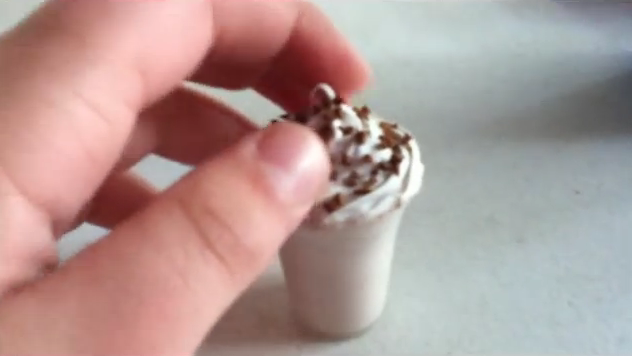
\includegraphics[width=\textwidth]{troll_1.png}
  \end{subfigure}~
  \begin{subfigure}[b]{0.16\textwidth}
    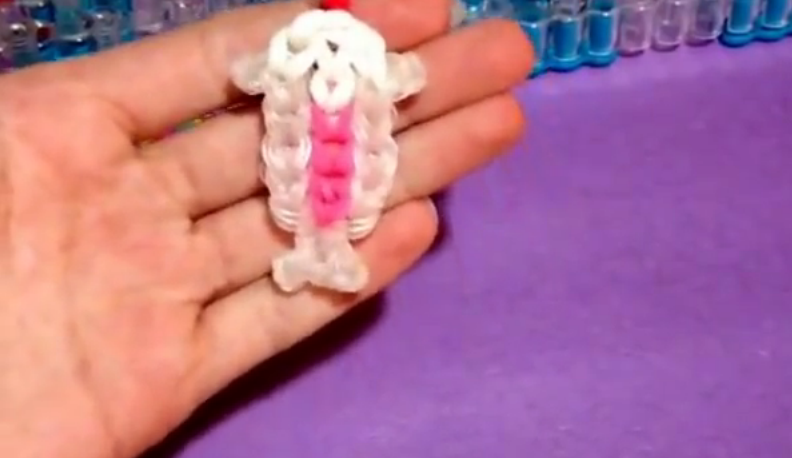
\includegraphics[width=\textwidth]{troll_2.png}
  \end{subfigure}~
  \begin{subfigure}[b]{0.16\textwidth}
    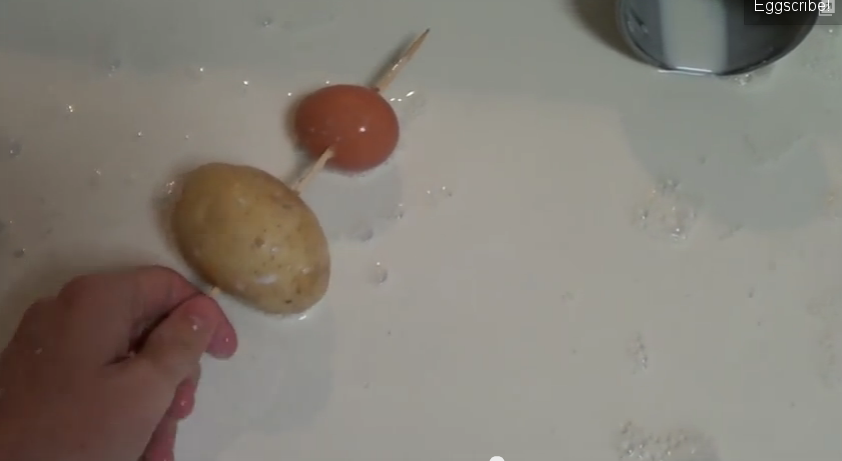
\includegraphics[width=\textwidth]{troll_3.png}
  \end{subfigure}
\caption{\textbf{Sample videos which our algorithm discards as an outlier for the query \emph{How to make a milkshake?}.} These videos are about a toy milkshake, a milkshake charm and a funny video about How to NOT make milkshakes.}
\label{outliers}
\end{figure}

\subsection{Semantic Multi-Modal Frame Representation}
We represent the each frame of the each video by using set of language and visual atoms which we automatically extract. Language atoms are the salient words learned by ranking the words in the subtitle corpus via tf-idf like measure. And, the visual atoms are found by clustering over region proposals which we extract from each frame. We explain the details of proposal generation, clustering and ranking in the subsequent sections.

\subsubsection{Learning Language Atoms}
After obtaining the videos and subtitles belonging to a single query, we concatanate all subtitles into a single collection(term corpus). As a document, we use all the words extracted from all subtitles of all queries. Moreover, we compute the tf-idf as $tfidf(w,d,D)=f_{w,d} \times \log \frac{N}{n_{w}}$ where $w$ is the word, $d$ is the collection of words corresponding to the query, $f_{w,d}$ is the frequency of the word in the collection $d$, $N$ is the total number of videos returned from all queries and $n_{w}$ is the number of videos whose subtitle include the word $w$. After computing the tf-idf, we sort all words with their tf-idf values and choose the top $K$ words as set of salient words (\emph{We set $K=100$ in our experiments}).

We show below the top 50 salient words extracted for the query \emph{How to hard boil an egg?}. Moreover, they correspond to important objects, actions and adjectives which can semantically relate actions over multiple videos.

\footnotesize
\emph{sort, place, water, egg, bottom, fresh, pot, crack, cold, cover, time, overcooking, hot, shell, stove, turn, cook, boil, break, pinch, salt, peel, lid, point, haigh, rules, perfectly, hard, smell, fast, soft, chill, ice, bowl, remove, aside, store, set, temperature, coagulates, yolk, drain, swirl, shake, white, roll, handle, surface, flat}
\normalsize


\subsubsection{Learning Visual Atoms}
In order to learn visual atoms, we create a large collection of proposals by independently generating region proposals from each frame of the each video. These proposals are generated by using the Constrained Parametric Min-Cut (CPMC) \cite{cpmc} algorithm by using both apperance and motion cues. We note the $k^{th}$ region of $t^{th}$ frame of $i^{th}$ video as $r^{(i),k}_t$. Moreover, we drop the video index $(i)$ if it is clear from the context.

We follow the spectral graph clustering approach in order to group these regions into semantically meaningful objects similar to the Keysegments approach \cite{keysegments}. However, idea of clustering region proposals into set of semantic objects have been mostly utilizied for clusters generated by a single video and they fail to cluster objects having a large visual difference. Hence, we extend this work to spectral joint clustering of region proposals over multiple videos.

\paragraph{Joint Proposal Clustering to Detect Visual Objects}
Since our proposals are generated from multiple videos, combining them into a single region collection and clustering it is not desired for two reaons; (1) objects have large visual differences among videos and accurately clustering them into a single cluster is hard, (2) clusters are desired to have region proposals from multiple videos in order to semantically relate videos. We propose a joint version of the spectral region clustering algorithm to satisfy these requirements.

\begin{figure}[ht]
  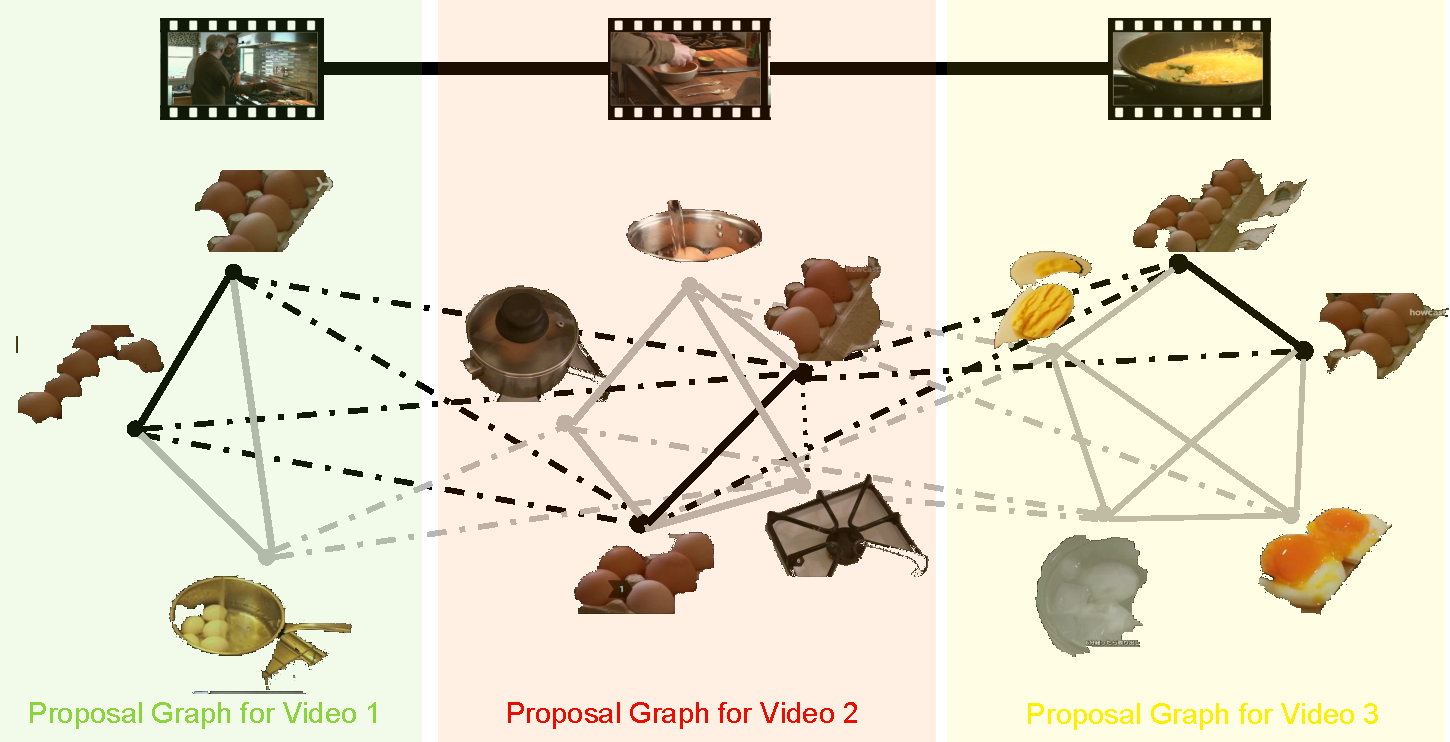
\includegraphics[width=0.48\textwidth]{joint_clustering}
  \scalebox{0.85}{$\arg\max  \color[HTML]{BF9000}{\frac{x_1^TA^{(1)}x^1}{x_1^Tx^1}}+\color[HTML]{990000}{\frac{x_2^TA^{(2)}x^2}{x_2^Tx^2}}+\color[HTML]{38761d}{\frac{x_3^TA^{(3)}x^3}{x_3^Tx^3}}+\color[HTML]{a64d79}{\frac{x_1^TA^{(1,2)}x^2}{x_1^T\mathds{1}\mathds{1}^Tx^2}}+\color[HTML]{F1C232}{\frac{x_2^TA^{(2,3)}x^3}{x_2^T\mathds{1}\mathds{1}^Tx^3}}$}
  \caption{\textbf{Visualization of the joint proposal clustering.} Here, we show the 1NN video graph and 2NN region graph. Each region proposal is linked to its 2 nearest neihbours from the video it belongs and 2 nearest neighbours from the videos it is neighbour of.}
  \label{hierProposal}
\end{figure}

We first explain the original spectral graph clustering algorithm and then extend it to joint clustering. Consider the set of region proposals extracted from a single video $r^k_t$, and a similarity metric $d(\cdot,\cdot)$ between any region proposal pair. We follow the single cluster graph partitioning (SCGP)\cite{scgp} approach to find the dominant cluster which maximizes the inter-cluster similarity. In other words, we solve
\begin{equation}
  \argmax_{x^k_t} \frac{\sum_{(k_1,t_1),(k_2,t_2) \in K \times T} x^{k_1}_{t_1} x^{k_2}_{t_2} d(r^{k_1}_{t_1},r^{k_2}_{t_2})}{\sum_{(k,t) \in K \times T} x^{k}_t}
\end{equation}
where, $x^{k}_t$ is a binary variable which is $1$ if $r^{k}_t$ is included in the cluster, $T$ is the number of frames and $K$ is the number of clusters per frame. When we use the vector form of the indicator variables as $\mathbf{x_{tK+k}}=x^{k}_{t}$ and the pairwise distance matrix as $\mathbf{A}_{t_1K+k_1,t_2K+k_2}=d(r^{k_1}_{t_1},r^{k_2}_{t_2})$, this equation can be compactly written as
$\argmax_{\mathbf{x}} \frac{\mathbf{x^T}A\mathbf{x}}{\mathbf{x^T}\mathbf{x}}$
Moreover, it can be solved by finding the dominant eigenvector of $\mathbf{x}$ after relaxing $x^{k}_t$ to $[0,1]$ \cite{scgp,scgp_eigen}. After finding the maximum, the remaining clusters can be found by removing the selected region proposals from the collection, and re-aplying the same algorithm for the second dominant cluster.

Our extension of the SCGP into multiple videos is based on the assumption that the important objects of recipes occur in most of the videos. Hence, we re-formulate the problem by relating videos to each other. We use the kNN graph of the videos which we used for the outlier detection as explained in the Section~\ref{outlier}. Moreover, we also create the kNN graph of region proposals in each video. This hierarchical graph structure is also visualized in Figure~\ref{hierProposal} for 3 videos. After creating this graph, we impose the similarity of regions in the selected cluster coming from each video as well as the similarity of regions coming from neighbour videos. Hence, given the pairwise distance matrices $\mathbf{A^{(i)}}$, binary indicator vectors $\mathbf{x^{(i)}}$ for each video and pairwise distance matrices for video pairs as $\mathbf{A^{(i,j)}}$, we define our optimization problem as;
\begin{equation}
\argmax \sum_{i \in N} \frac{\mathbf{x^{(i)^T}}\mathbf{A^{(i)}}\mathbf{x^{(i)}}}{\mathbf{x^{(i)^T}}\mathbf{x^{(i)}}} +
\sum_{i \in N} \sum_{j \in \mathcal{N}(i)} \frac{\mathbf{x^{(i)^T}}\mathbf{A^{(i,j)}}\mathbf{x^{(j)}}} {\mathbf{x^{(i)^T}}\mathds{1}\mathds{1}^T\mathbf{x^{(j)}}}
\end{equation}
where $\mathcal{N}(i)$ is the neighbours of the video $i$ in the kNN graph, $\mathds{1}$ is vector of ones and $N$ is the number of videos. We visualize this optimization objective in Figure~\ref{hierProposal} for the case of 3 videos.

After changing the optimization function, we can not use the efficient eigen-decomposition based approach from \cite{scgp,scgp_eigen}; however, we can use stochastic gradient descent (SGD) since the cost function is quasi-convex when it is relaxed. We use the SGD with the following gradient function;
\begin{equation}
  \nabla_{\mathbf{x^{(i)}}} = \frac{2\mathbf{A^{(i)}} \mathbf{x^{(i)}} -2\mathbf{x^{(i)}} r^{(i)}}
  {\mathbf{{x^{(i)}}^T}\mathbf{x^{(i)}}}
+ \sum_{i \in N} \frac{\mathbf{A^{i,j}}\mathbf{x^{j}} - \mathbf{{x^{(j)}}^T} \mathds{1} r^{(i,j)}}{\mathbf{{x^{(i)}}^T} \mathds{1} \mathds{1}^T \mathbf{x^{(j)}} }
  %\text{Some vector matrix multiplication}
\end{equation}

where $r^{(i)}=\frac{\mathbf{x^{(i)^T}}\mathbf{A^{(i)}}\mathbf{x^{(i)}}}{\mathbf{x^{(i)^T}}\mathbf{x^{(i)}}}$ and $r^{(i,j)}=\frac{\mathbf{x^{(i)^T}}\mathbf{A^{(i,j)}}\mathbf{x^{(j)}}} {\mathbf{x^{(i)^T}}\mathds{1}\mathds{1}^T\mathbf{x^{(j)}}}$

In Figure~\ref{cvis}, we visualize some of the clusters which our algorithm generated after applied on the videos returned by the query \emph{How to Hard Boil an Egg}. As shown the figure, the resulting clusters are highly correlated and correspond to semantic objects\&concepts.
\begin{figure}[ht]
  \begin{subfigure}[b]{0.23\textwidth}
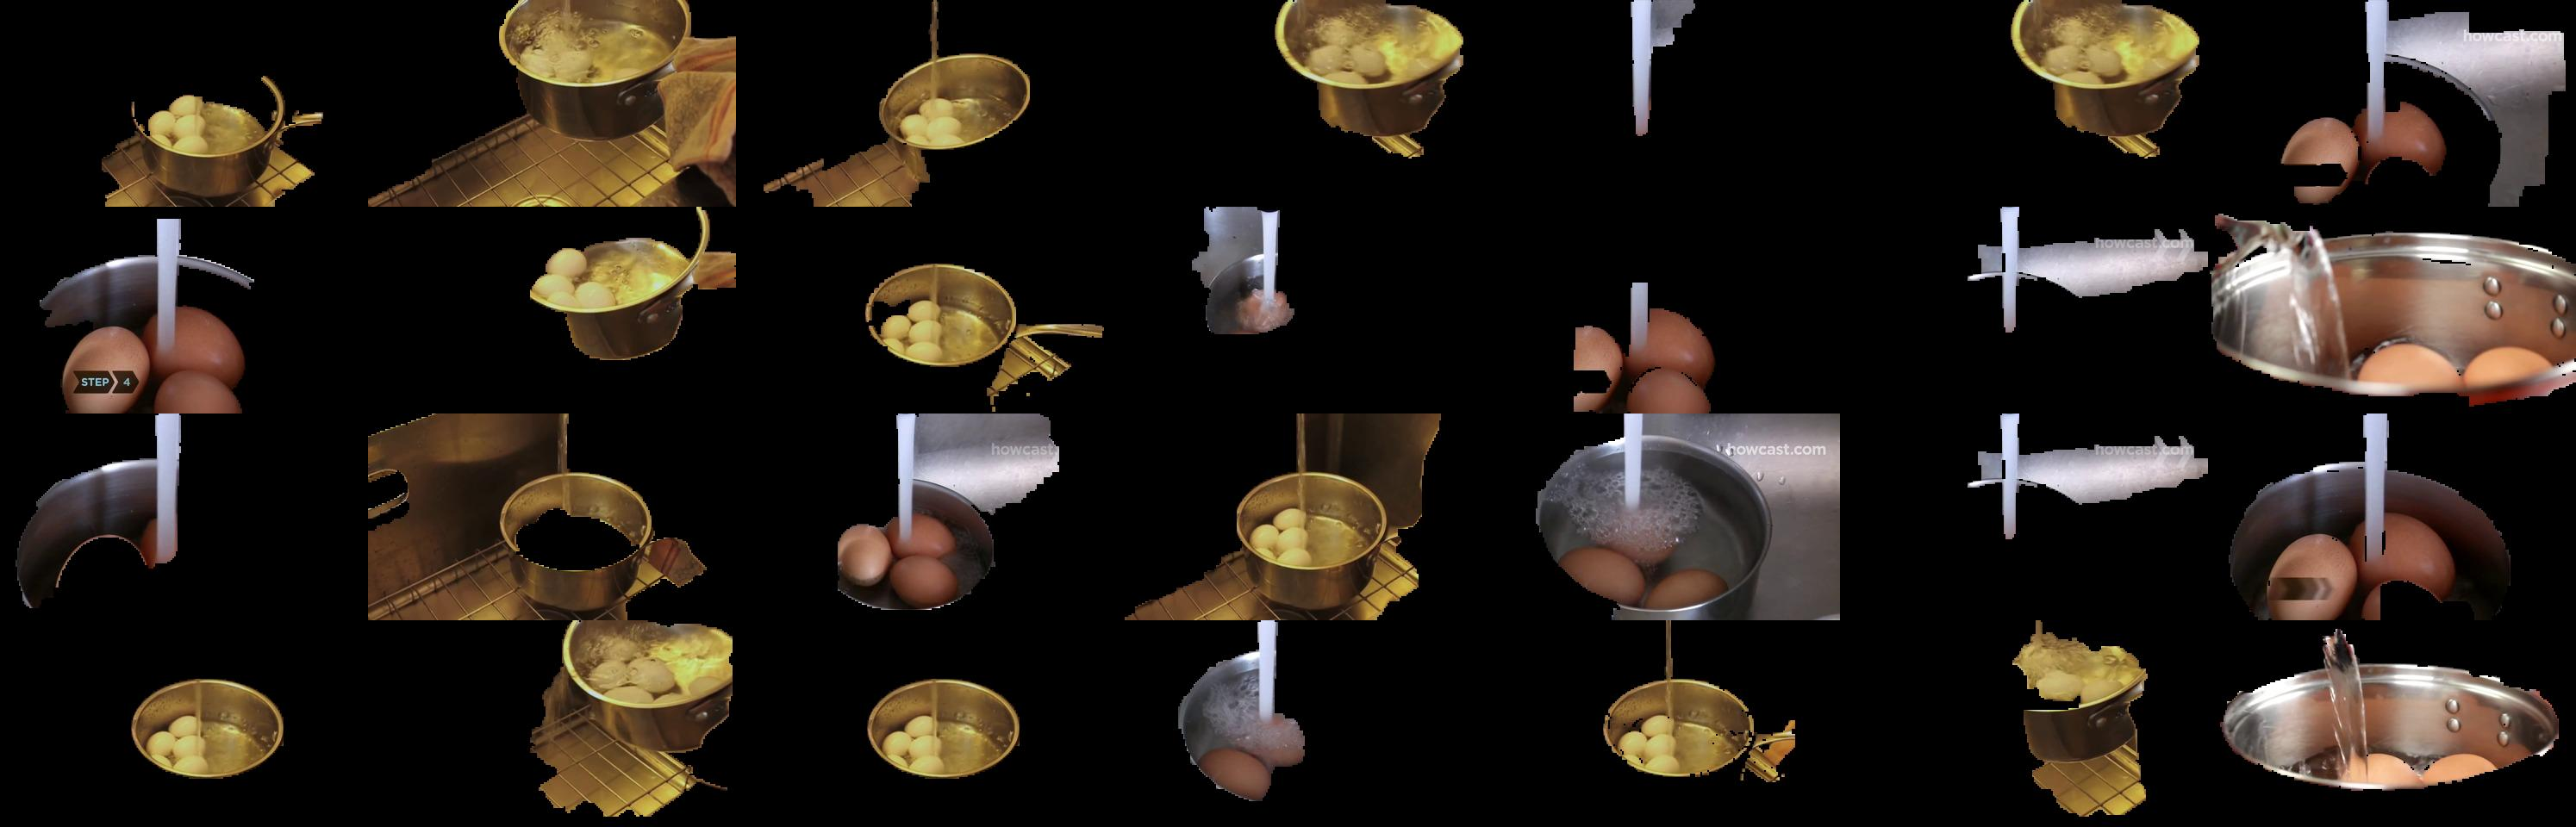
\includegraphics[width=\textwidth]{im0.png}
%\caption{Cluster 1}
\end{subfigure}
~
\begin{subfigure}[b]{0.23\textwidth}
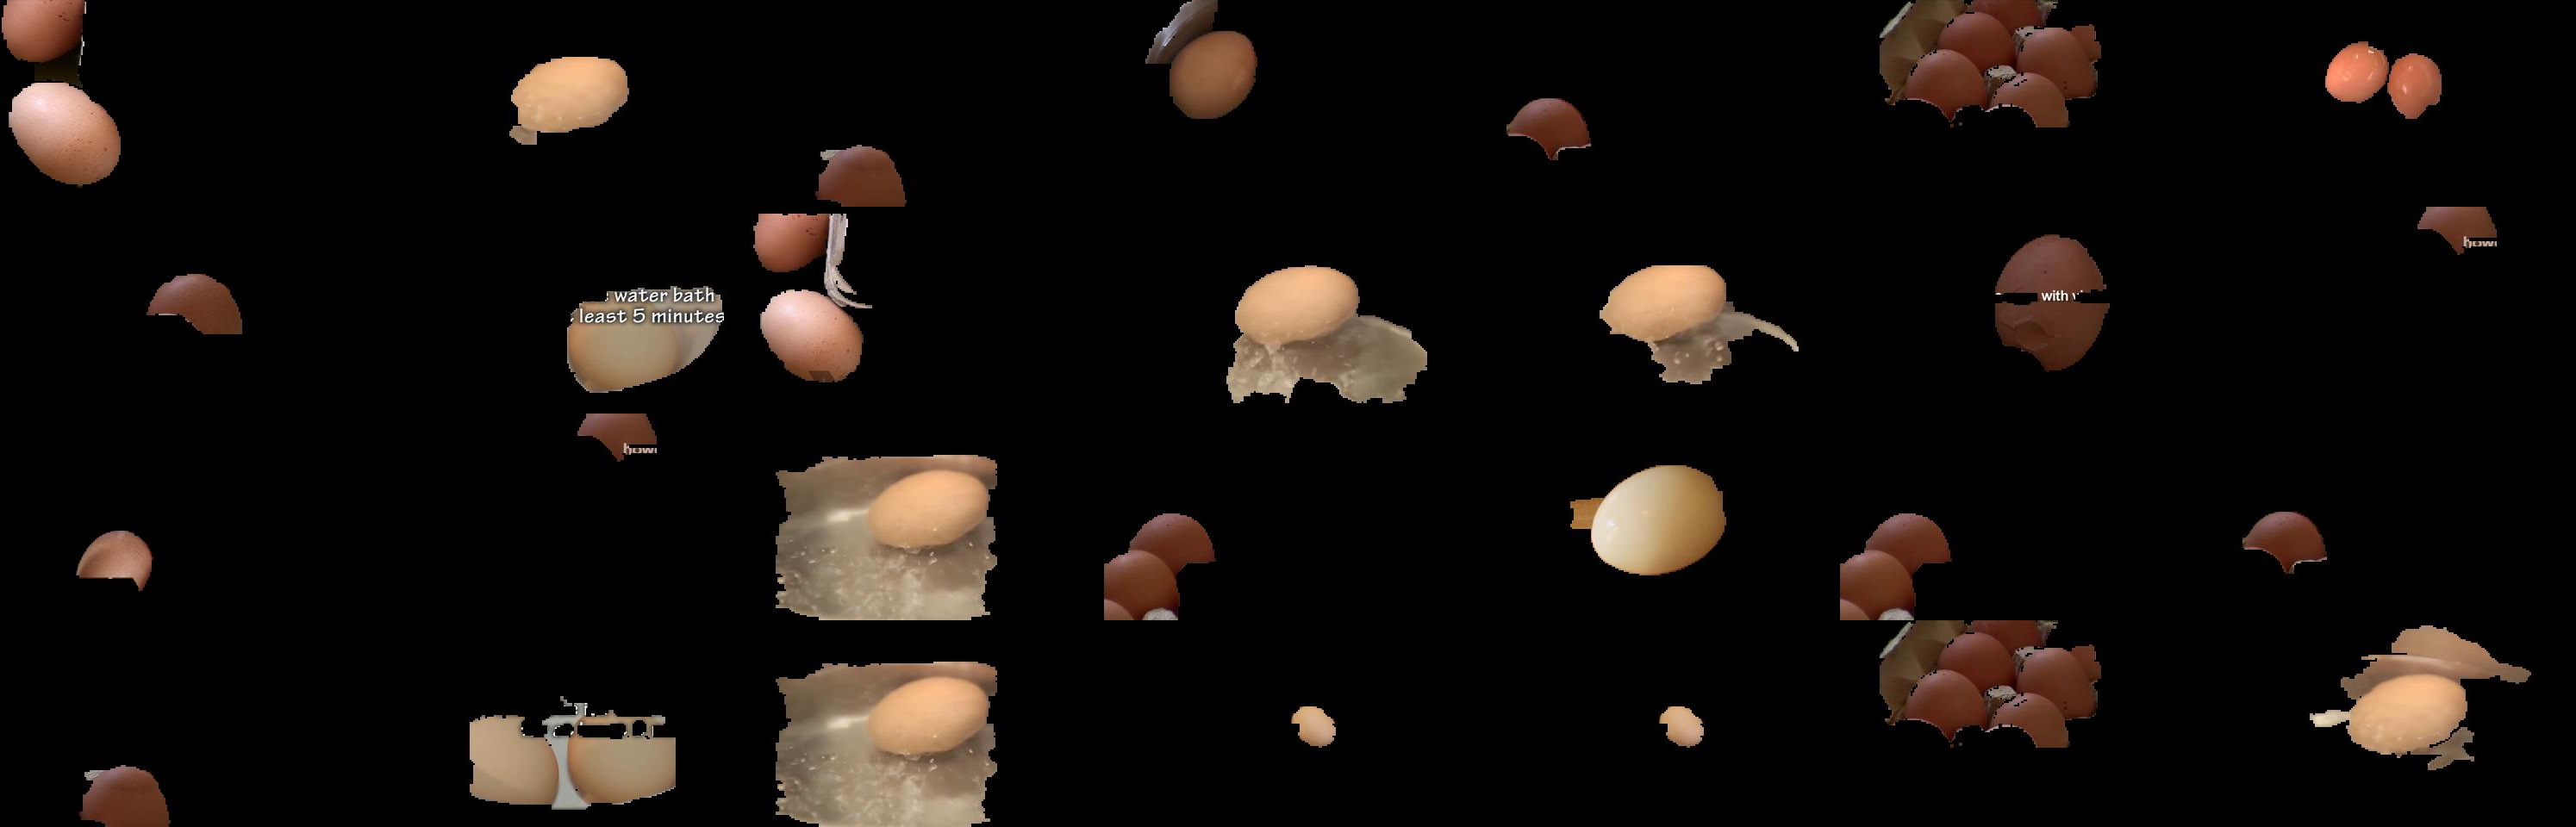
\includegraphics[width=\textwidth]{im4.png}
%\caption{Cluster 2}
\end{subfigure}
\begin{subfigure}[b]{0.23\textwidth}
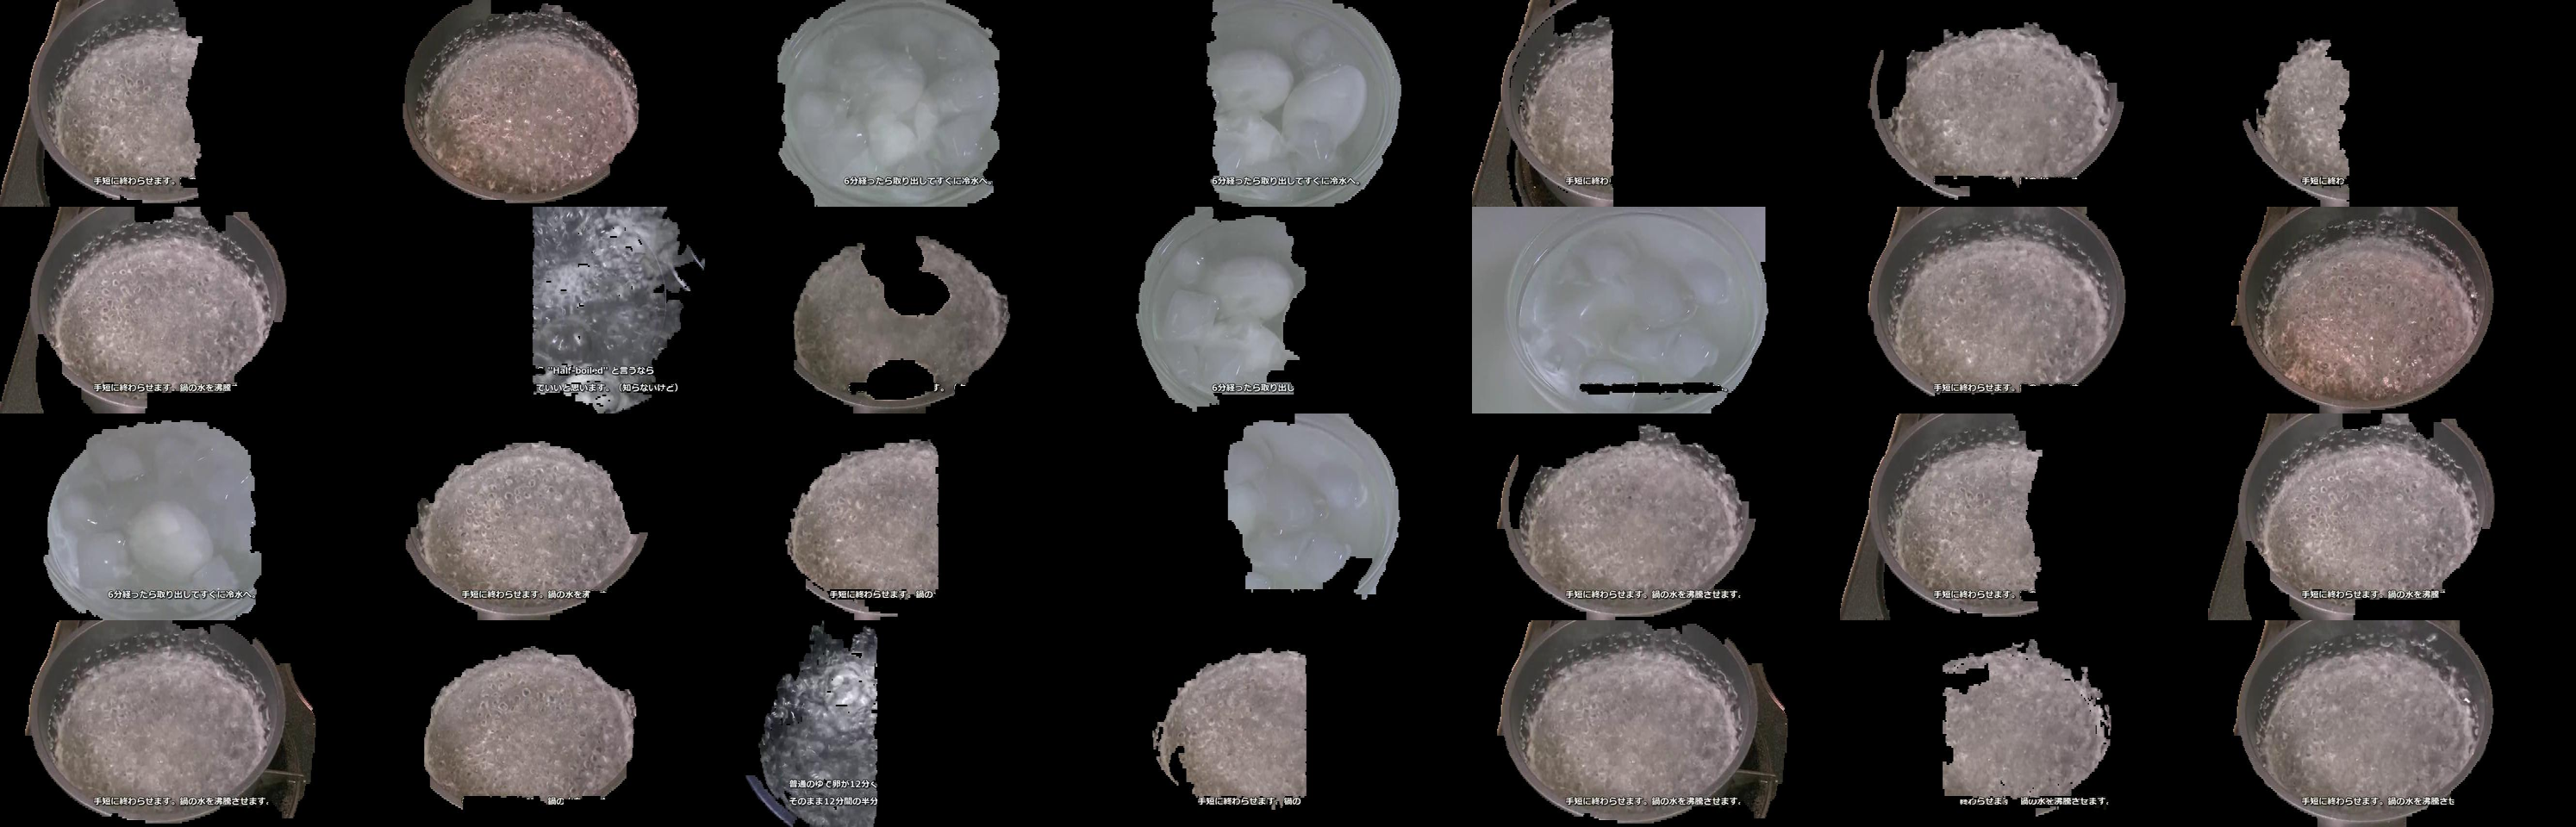
\includegraphics[width=\textwidth]{im5.png}
\end{subfigure}
~
\begin{subfigure}[b]{0.23\textwidth}
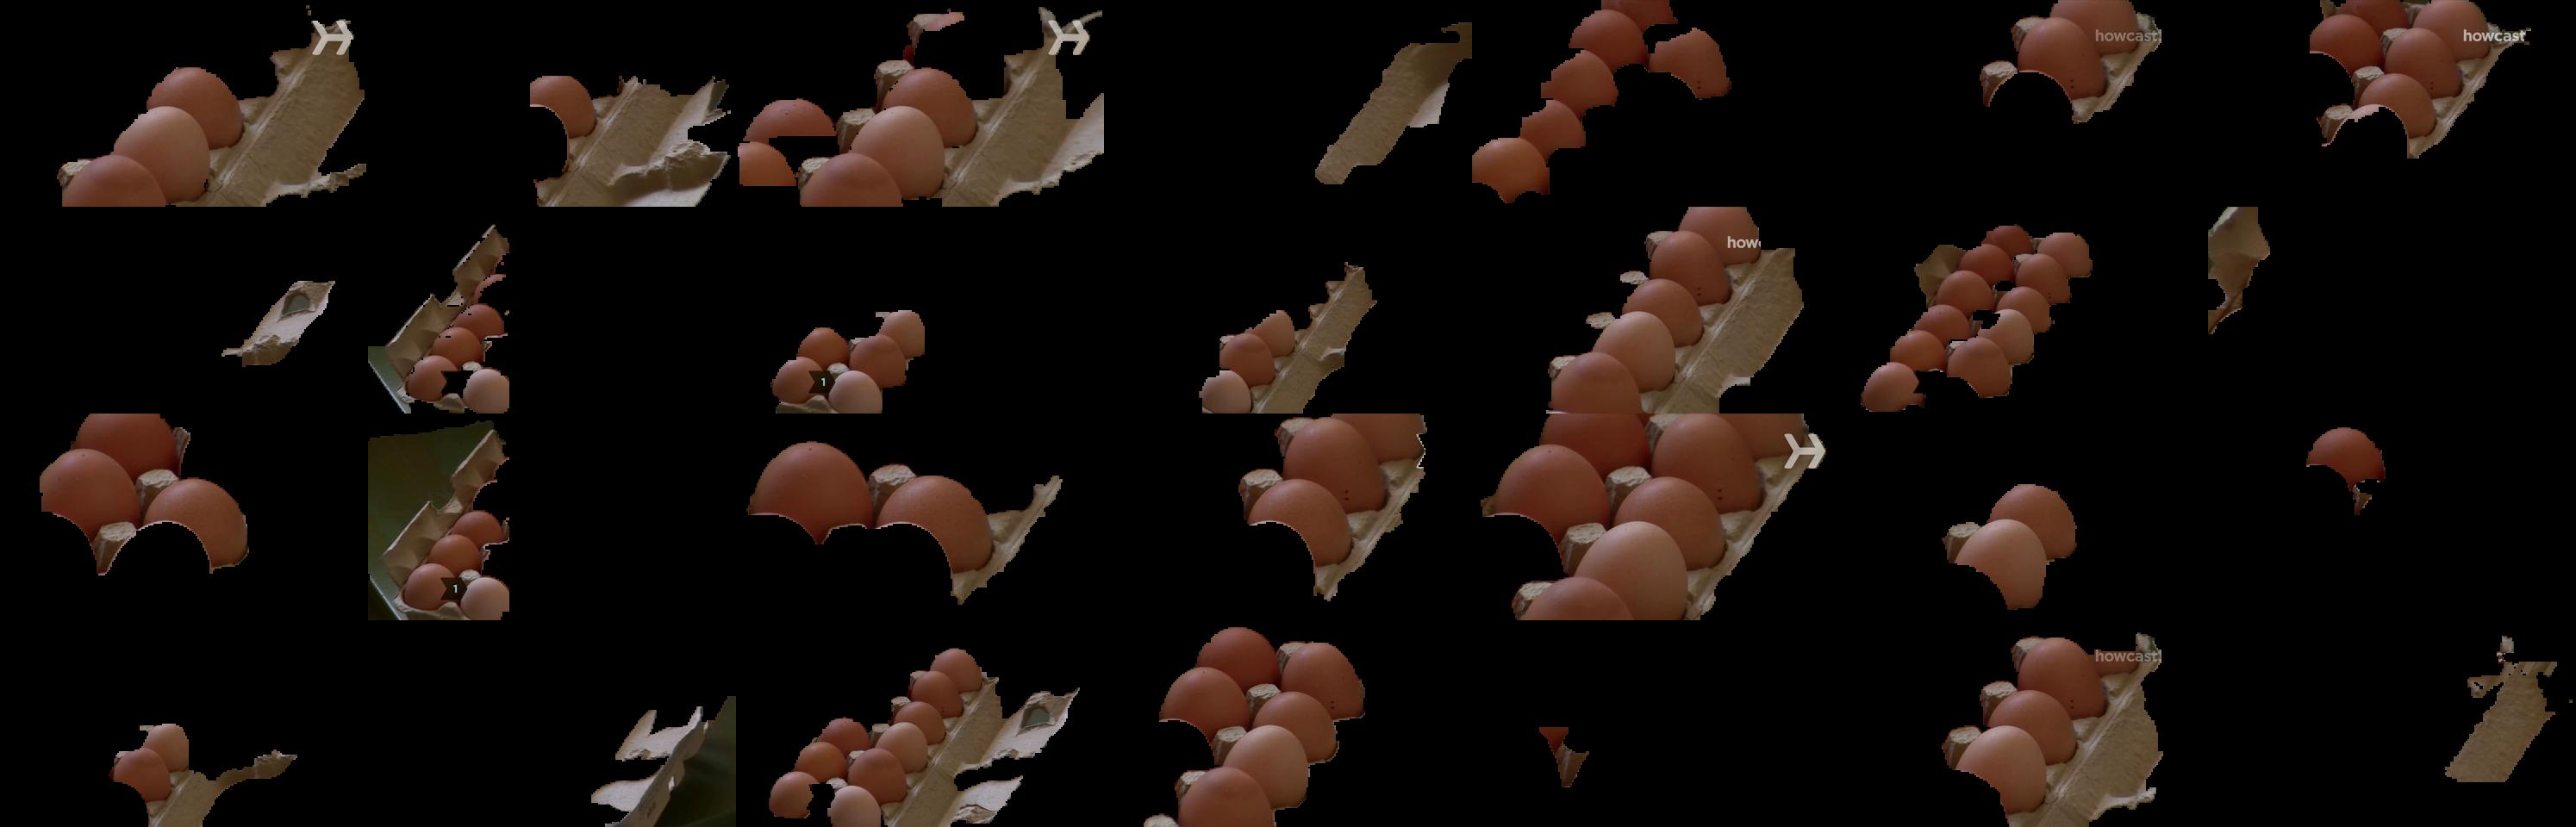
\includegraphics[width=\textwidth]{im7.png}
\end{subfigure}

\begin{subfigure}[b]{0.23\textwidth}
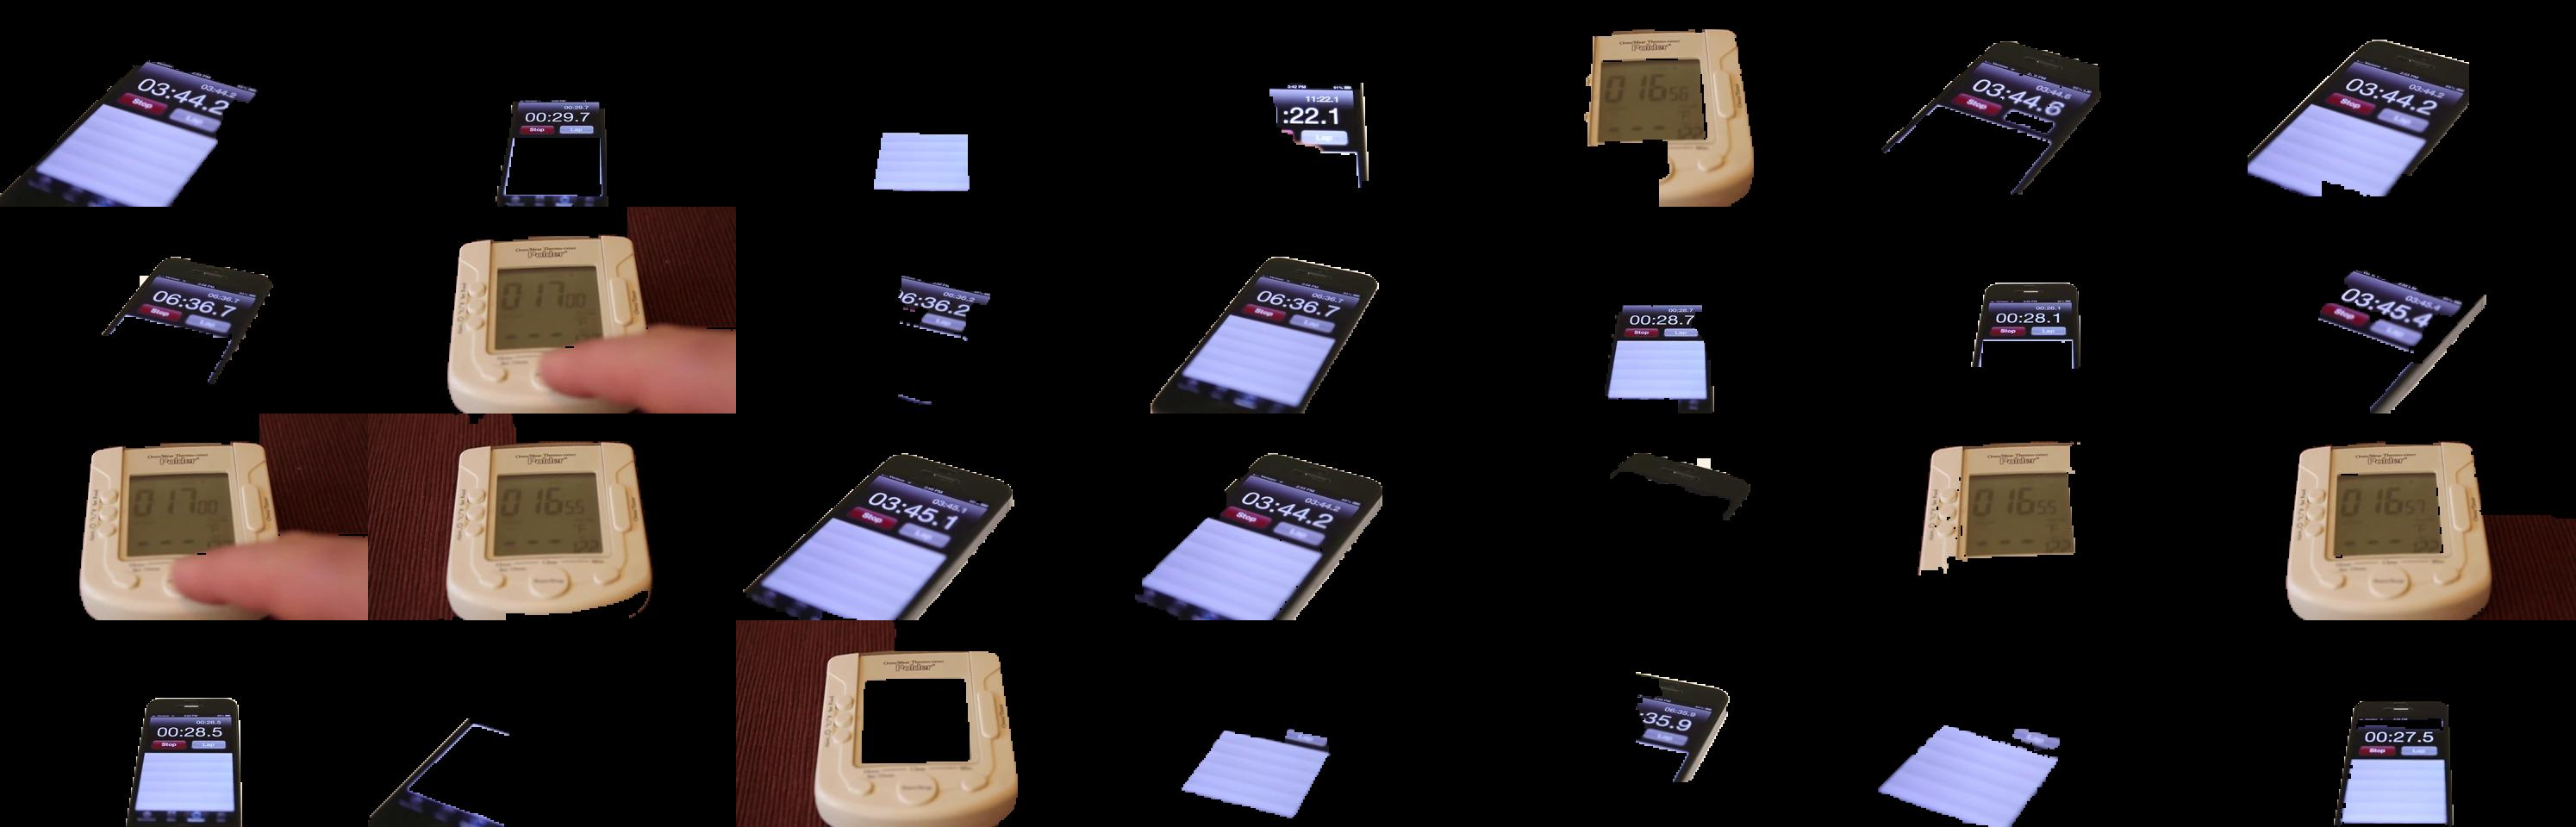
\includegraphics[width=\textwidth]{im8.png}
\end{subfigure}
~
\begin{subfigure}[b]{0.23\textwidth}
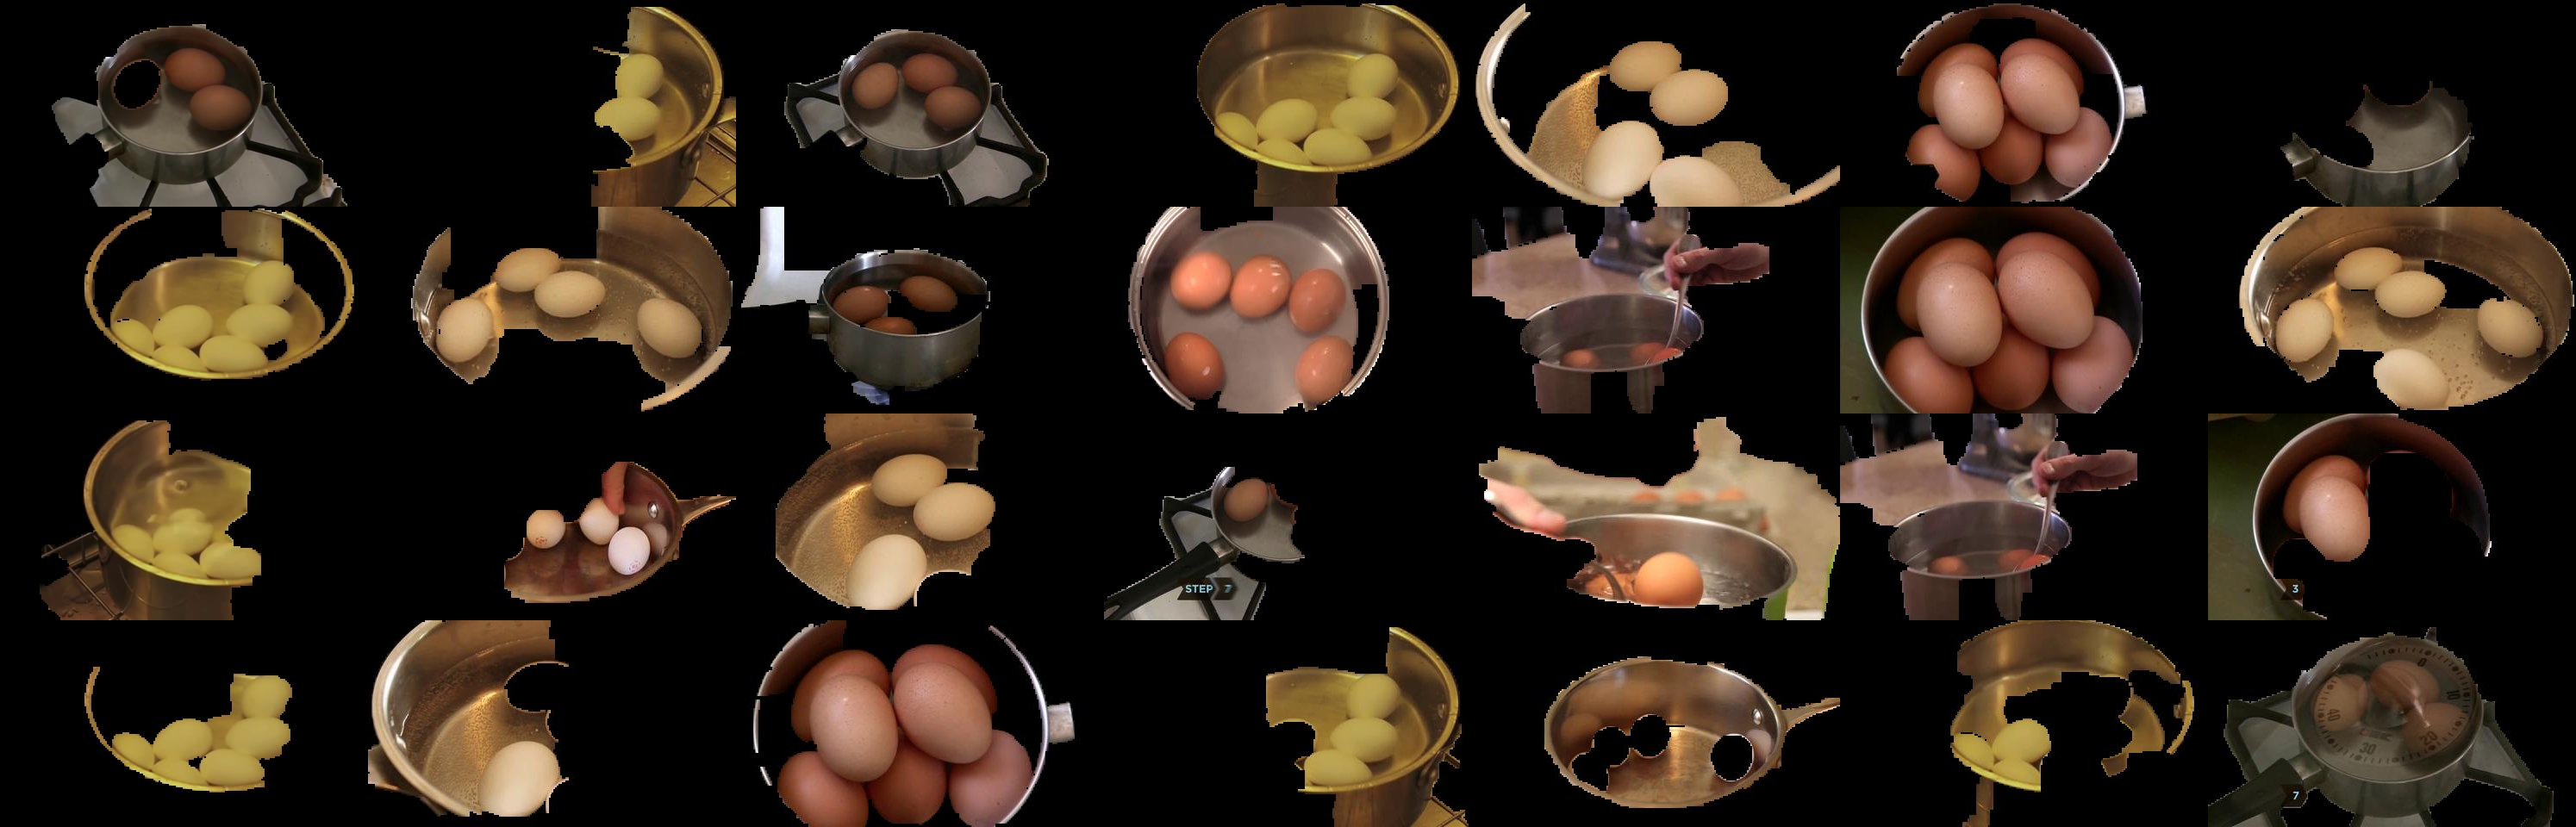
\includegraphics[width=\textwidth]{im10.png}
\end{subfigure}
\caption{Randomly selected images of randomly selected clusters learned for \emph{How to boil an egg?}}
\label{cvis}
\end{figure}
\subsection{Multi-Modal Representation via Learned Atoms}

\subsection{Unsupervised Activity Representation}
\label{basics}
\label{learning}
In this section, we explain the model which we use to discover the activity steps from a video collection given the language and visual atoms. We note the extracted representation of the frame $t$ of video $i$ as $\mathbf{y^{(i)}_t}$. We model our algorithm based on activity steps and note the activity label of the $t^{th}$ frame of the $i^{th}$ video as $z^{(i)}_t$. We do not fix the the number of activities and use a non-parametric approach.

%We start with explaining the notation. As we already defined in the previous sections,

In our model, each activity step is represented over the atoms as the likelihood of including them. In other words, each activity step is a Bernoulli distribution over the visual and language atoms as $\theta_k=[\theta_k^l,\theta_k^v]$ such that $m^{th}$ entry of the $\theta_k^l$ is the likelihood of observing $m^{th}$ language atom in the frame of an activity $k$. Similarly, $m^{th}$ entry of the $\theta_k^v$ represents the likelihood of seeing $m^{th}$ visual atom. In other words, each frame's representation $\mathbf{y^{(i)}_t}$ is sampled from the distribution corresponding to its activity as \mbox{$\mathbf{y^{(i)}_t}|z^{(i)}_t=k \sim Ber(\theta_k)$}. As a prior over $\theta$, we use its conjugate distribution -- \emph{Beta distribution} --.

Given the model above, we explain the generative model which links activity steps and frames in Section~\ref{bphmm}.
 %The key idea is each frame is represented via atoms and each activity step is a distribution over atoms hence the atoms are the linkage. We further explain the learning method to fit this model without any supervision in the Section~\ref{gibbs}.
\subsubsection{Beta Process Hidden Markov Model}
\label{bphmm}
For the understanding of the time-series information, Fox et al.\cite{foxBPHMM} proposed the Beta Process Hidden Markov Models (BP-HMM). In BP-HMM setting, each time-series exhibits a subset of available features. Similarly, in our setup each video exhibits a subset of activity steps.
%It is based on the notion features(\eg activity steps) which can explain the behaviour of a collection of time-series data (\eg video collection).

Our model follows the construction of Fox et al.\cite{foxBPHMM} and differs in the choice of probability distributions since \cite{foxBPHMM} considers Gaussian observations while we adopt binary observations of atoms. In our model, each video $i$ chooses a set of activity steps through an activity step vector $\mathbf{f^{(i)}}$ such that $f^{(i)}_k$ is $1$ if $i^th$ video has the activity step $k$, and 0 otherwise. When the activity step vectors of all videos are concatenated, it becomes an activity step matrix $\mathbf{F}$ such that $i^th$ row of the $\mathbf{F}$ is the activity step vector $\mathbf{f^{(i)}}$. Moreover, each activity step $k$ also has a prior probability $b_k$  and a distribution parameter $\theta_k$ which is the Bernoulli distribution as we explained in the Section~\ref{basics}.

In this setting, the activity step parameters $\theta_k$ and $b_k$ follow the \emph{beta process} as;
\begin{equation}
  B|B_0,\gamma,\beta \sim \text{BP}(\beta,\gamma B_o), B=\sum_{k=1}^\infty b_k \delta_{\theta_k}
\end{equation}
where $B_0$ and the $b_k$ are determined by the underlying Poisson process \cite{ibp} and the feature vector is determined as independent Bernoulli draws as $f_{k}^{(i)} \sim Ber(b_k)$. After marginalizing over the $b_k$ and $\theta_k$, this distribution is shown to be equivalent to Indian Buffet Process (IBP)\cite{ibp}. In the IBP analogy, each video is a customer and each activity step is a dish in the buffet. The first customer (video) chooses a $\text{Poisson}(\gamma)$ unique dishes (activity steps). The following customer (video) $i$ chooses previously sampled dish (activity step) $k$ with probability $\frac{m_k}{i}$,  proportional to the number of customers ($m_k$) chosen the dish $k$, and it also chooses $\text{Poisson}(\frac{\gamma}{i})$ new dishes(activity steps). Here, $\gamma$ controls the number of selected activities in each video and $\beta$ promotes the activities getting shared by videos.

The above IBP construction represents the activity step discovery part of our method. In addition, we also need to model the video parsing over discovered steps. Moreover, we need to model this two steps jointly. We model the each video as an Hidden Markov Model (HMM) over the selected activity steps. Each frame has the hidden state --activity step-- ($z^{(i)}_t$) and we observe the multi-modal frame representation $\mathbf{y^{(i)}_t}$. Since we model each activity step as a Bernoulli distribution, the emission probabilities follow the Bernoulli distribution as $p(\mathbf{y^{(i)}_t}|z^{(i)}_t)=Ber(\theta_{z^{(i)}_t})$.

For the transition probabilities of the HMM, we do not put any constraint and simply model it as any point from a probability simplex which can be sampled by drawing a set of Gamma random variables and normalizing them \cite{foxBPHMM}. For each video $i$, a Gamma random variable is sampled for the transition between activity step $j$ and activity step $k$ if both of the activity steps are included by the video (\ie if $f^i_k$ and $f^i_j$ are both $1$). After sampling these random variables, we normalize them to make transition probabilities to sum up 1. This procedure can be represented formally as
\begin{equation}
  \eta_{j,k}^{(i)} \sim Gam(\alpha+\kappa \delta_{j,k},1), \quad \mathbf{\pi_j^{(i)}} = \frac{\mathbf{\eta^{(i)}_j} \circ \mathbf{f^{(i)}}}{\sum_k \eta^{(i)}_{j,k} f^{(i)}_k}
\end{equation}
Where $\kappa$ is the persistence parameter promoting the self state transitions a.k.a. more coherent temporal boundaries, $\circ$ is the element-wise product and $\pi^i_j$ is the transition probabilities in video $i$ from activity step $j$ to other steps. This model is also presented as a graphical model in Figure \ref{bphmmo}
\begin{figure}[h!]
  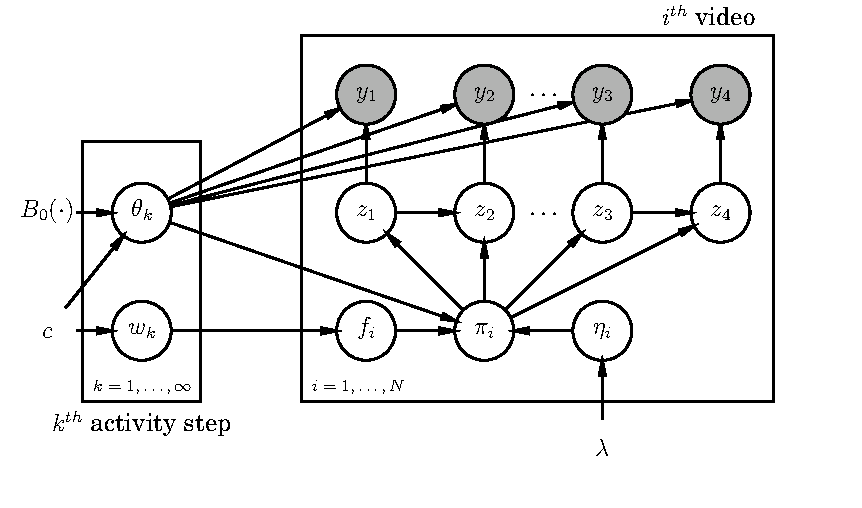
\includegraphics[width=0.5\textwidth]{plate}
  \vspace{-9mm}
  \caption{\textbf{Graphical model for BP-HMM:} The left plate represent the activity steps and the right plate represent the videos. \ie the left plate is for the activity step discovery and right plate is for parsing. \emph{See Section~\ref{bphmm} for details.}}
  \vspace{-5mm}
  \label{bphmmo}
\end{figure}


\subsubsection{Gibbs sampling for BP-HMM}
We employ Markov Chain Monte Carlo (MCMC) method for learning and inference of the BP-HMM. We base our algorithms on the MCMC procedure proposed by Fox et al.\cite{foxBPHMM}. Our sampling procedure composed of two samplers: (1) activity step ($\mathbf{f^{(i)}}$) sampler from the current activity step distributions $\mathbf{\theta_k}$ and multi-modal frame representations $y^{(i)}_k$, (2) and HMM parameter $\mathbf{\eta}$,$\mathbf{\pi}$,$\mathbf{\theta_k}$ sampler from the selected activities $\mathbf{f^{(i)}}$. Intuitively, we iterate over discovering activity steps given the temporal activity labels and estimating activity labels given the discovered activities. We give the details of this sampler in supplementary material.

\section{Experiments}
In order to experiment the proposed method, we first collected a dataset (details in Section~\ref{dataset:sec}). We labelled small part of the dataset with frame-wise activity step labels and used the resulting set as an evaluation corpus. Neither the set of labels, nor the temporal boundaries are exposed to our algorithm since the set-up is completely unsupervised. We evaluate our algorithm against the several unsupervised clustering baselines and state-of-the-art algorithms from video summarization literature which are applicable.
\subsection{Dataset}
\label{dataset:sec}
We use WikiHow\cite{wikiHow} in order to obtain the top100 queries the internet users are interested in and choose the ones which are directly related to the physical world. In other words, we ignore queries like \emph{How to get over a break up‏?‎} as they have no objective set of steps. Resulting queries are;


\emph{\textbf{How to}}\footnotesize
\emph{Bake Boneless Skinless Chicken, Make Jello Shots, Cook Steak, Bake Chicken Breast, Hard Boil an Egg, Make Yogurt, Make a Milkshake, Make Beef Jerky, Tie a Tie, Clean a Coffee Maker, Make Scrambled Eggs, Broil Steak, Cook an Omelet, Make Ice Cream, Make Pancakes, Remove Gum from Clothes, Unclog a Bathtub Drain}
\normalsize

For each of the queries, we crawled YouTube and got the top 100 videos. We also downloaded the English subtitles if they exist. For evaluation set, we randomly choose 5 videos out of 100 per query. Hence, we have total of 125 evaluation videos and 2375 unlabelled videos. We label the start and end frames of activity steps as well as the name of the step. We will release the code and collected dataset.

\subsubsection{Outlier Detection}
\label{filter}
Since we do not have any expert intervention in our data collection, the resulting collection might have outliers. Main reason for the outliers are  the fact that our queries are typical daily activities and there are many cartoons, funny videos, and music videos about them. Hence, we have an automatic filtering stage. The key-idea behind the filtering algorithm is the fact that instructional videos have a distinguishable text descriptions when compared with outliers. Hence, we use a clustering algorithm to find the large cluster of instructional videos. Given a large video collection, we use the graph we explain in Section~\ref{jointProp} and compute the dominant video cluster by using the Single Cluster Graph Partitioning \cite{scgp} and discards the remaining videos as outlier. In Figure~\ref{outliers}, we visualize some of the discarded videos. Although our algorithm have false positives while detecting outliers, we always have enough number of videos (minimum 50) after the outlier detection thanks to the large-scale dataset.

\begin{figure}[ht]
%  \begin{subfigure}[b]{0.5\textwidth}
    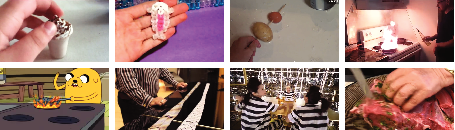
\includegraphics[width=0.5\textwidth]{figure_7_flt}
%  \end{subfigure}~
\caption{\textbf{Sample videos which our algorithm discards as an outlier for various queries.}
A toy milkshake, a milkshake charm, a funny video about How to NOT make smoothie, a video about the danger of a fire, a cartoon video, a neck-tie video erroneously labeled as bow-tie, a song, and a lamb cooking mislabeled as chicken.}
\label{outliers}
\vspace{-3mm}
\end{figure}

\subsection{Qualitative Results}
After independently running our algorithm on all categories, we discover activity steps and parse the videos according to discovered steps. We visualize some of these categories qualitatively in Figure~\ref{recipe:overall} with the temporal parsing of evaluation videos as well as the ground truth parsing.

To visualize the content of each activity step, we display key-frames from different videos. We also train a 3rd order Markov language model\cite{languageModel} by using the subtitles. Moreover, we generate a caption for each activity step by sampling this model conditioned on the $\theta^l_k$. We explain the details of this process in supplementary material.

\begin{figure*}[ht]
  \begin{subfigure}[b]{\textwidth}
    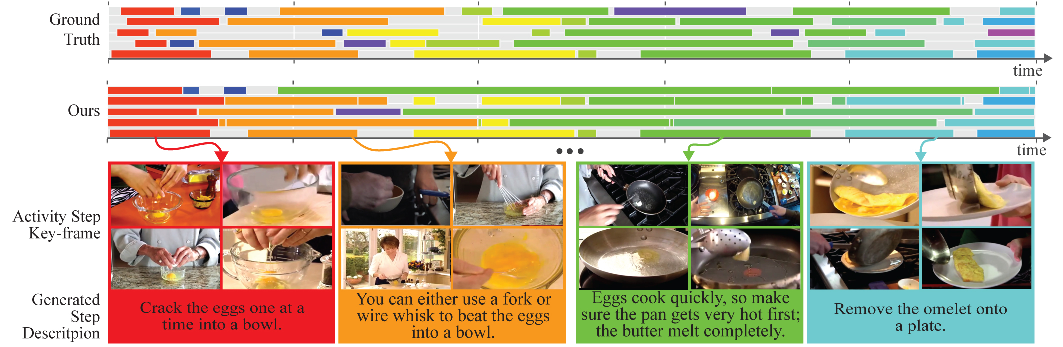
\includegraphics[width=\textwidth]{figure_8a_flattened}
    \vspace{-5mm}
    \caption{How to make an omelet?}
    \vspace{-1mm}
    \label{recipe:ommelette}
  \end{subfigure}

  \begin{subfigure}[b]{\textwidth}
    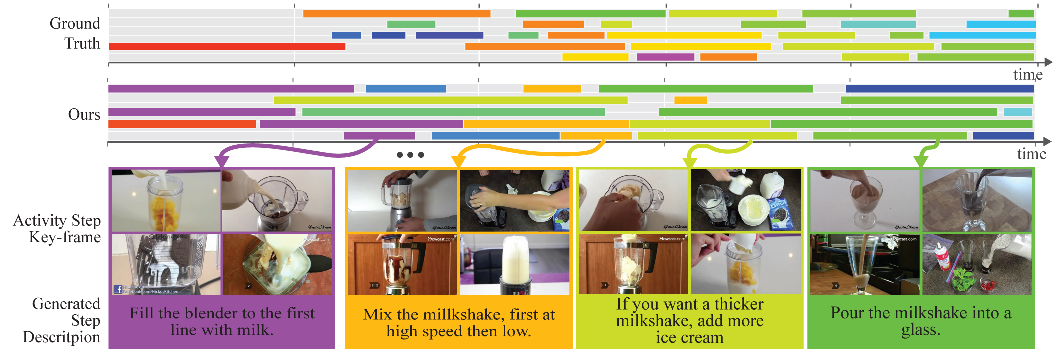
\includegraphics[width=\textwidth]{figure_8b_flattened}
    \caption{How to make a milkshake?}
    \vspace{-3mm}
    \label{recipe:milkshake}
  \end{subfigure}~
\caption{Temporal segmentation of the videos and ground truth segmentation. We also color code the activity steps we discovered and visualize their key-frames and the automatically generated captions. \emph{Best viewed in color.}}
\label{recipe:overall}
\vspace{-3mm}
%\normalsize}
\end{figure*}

As shown in the Figures~\ref{recipe:ommelette}\&\ref{recipe:milkshake}, resulting steps are semantically meaningful. Moreover, the language captions are also quite informative hence we can conclude that there is enough language context within the subtitles in order to detect activities. On the other hand, some of the activity steps always occur together and our algorithm merges them into a single step while promoting sparsity.

\subsection{Quantitative Results}
We compare our algorithm with the following baselines.

\noindent\textbf{Low-level features (LLF):}
In order to experiment the effect of learned atoms, we compare with low-level features. As features, we use the state-of-the-art Fisher vector representation of HOG, HOF and MBH features \cite{THUMOS14}.

\noindent\textbf{Single modality:}
To experiment the effect of multi-modal approach, we compare with single modality approach by only using the atoms of a single modality.

\noindent\textbf{Hidden Markov Model (HMM):}
To experiment the effect of joint generaive model, we compare our algorithm with an HMM. We use the Baum-Welch algorithm\cite{rabiner} and choose the number of clusters via cross-validation.


\noindent\textbf{Kernel Temporal Segmentation\cite{potapov2014category}:}
Kernel Temporal Segmentation (KTS) proposed by Potapov et al.\cite{potapov2014category} can detect the temporal boundaries of the events/activities in the video from a time series data without any supervision. It enforces a local similarity of each resultant segment.

\begin{figure*}[t]
  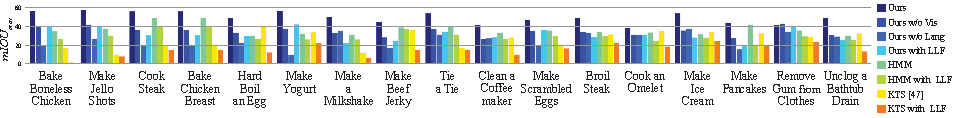
\includegraphics[width=\textwidth]{figure_9}
  \vspace{-9mm}
  \caption{$IOU_{max}$ values for all categories, for all competing algorithms.}
  \label{mIOU}
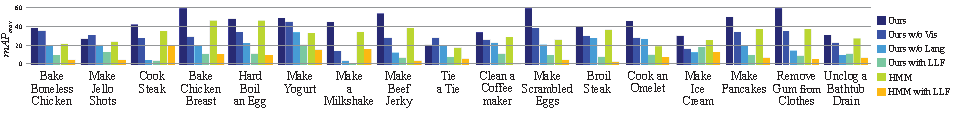
\includegraphics[width=\textwidth]{figure_10}
\vspace{-9mm}
\caption{$AP_{max}$ values for all categories, for all competing algorithms.}
\vspace{-3mm}
\label{mmAP}
\end{figure*}

Given parsing results and the ground truth, we evaluate both the quality of temporal segmentation and the activity step discovery. We base our evaluation on two widely used metrics; intersection over union ($IOU$) and mean average precision($mAP$). $\mathbf{IOU}$ measures the quality of temporal segmentation and it is defined as; $\frac{1}{N}\sum_{i=1}^N \frac{\tau^\star_i \cap \tau^\prime_{i}}{\tau^\star_i \cup \tau^\prime_{i}}$ where $N$ is the number of segments, $\tau^\star_i$ is ground truth  segment and $\tau^\prime_{i}$ is the detected segment. $\mathbf{mAP}$ is defined per activity step and can be computed based on a precision-recall curve \cite{THUMOS14}. In order to adopt these metrics into unsupervised setting, we use cluster similarity measure(csm)\cite{liao05} which enables us to use any metric in unsupervised setting. It chooses a matching of ground truth labels with predicted labels by searching over all matching and choosing the ones giving highest score. We use $mAP_{csm}$ and $IOU_{csm}$ as evaluation metrics.

\vspace{1mm}
\noindent\textbf{Accuracy of the temporal parsing.}
We compute, and plot in Figure\ref{mIOU}, the $IOU_{cms}$ values for all competing algorithms and all categories. We also average over the categories and summarize the results in the Table \ref{averM}. As the Figure~\ref{mIOU} and Table~\ref{averM} suggests, proposed method consistently outperforms the competing algorithms and its variations. One interesting observation is the importance of both modalities as a result of dramatic difference between the accuracy of our method and its single modal versions.

Moreover, the difference between our method and HMM is also significant. We believe this is due to the ill-posed definition of activities in HMM since the granularity of the activity steps is subjective. On the other hand, our method starts with the well-defined definition of finding set of steps which generate the entire collection. Hence, our algorithm do not suffer from granularity problem.
\begin{table}
\caption{Average of $IOU_{cms}$ and $mAP_{cms}$ over recipes.}
{\small
\resizebox{\columnwidth}{!}{%
\begin{tabular}{c|cc|cc|cccc}
 & KTS \cite{potapov2014category}    & KTS\cite{potapov2014category}     & HMM     & HMM    & Ours    & Ours     & Ours      & Our  \\
 &  w/ LLF &  w/ Sem &  w/ LLF &  w/Sem &  w/ LLF &  w/o Vis &  w/o Lang &  full \\
 \hline
$IOU_{cms}$  & 16.80 & 28.01      & 30.84 &   37.69   &  33.16 &  36.50 & 29.91& 52.36 \\
$mAP_{cms}$  &  n/a  & n/a        & 9.35  &   32.30   &  11.33 &  30.50 &  19.50 & 44.09 \\
\end{tabular}}}
\normalsize
\label{averM}
\vspace{-5mm}
\end{table}

\vspace{1mm}
\noindent\textbf{Coherency and accuracy of activity step discovery.}
Although $IOU_{cms}$ successfully measures the accuracy of the temporal segmentation, it can not measure the quality of discovered activities. In other words, we also need to evaluate the consistency of the activity steps detected over multiple videos. For this, we use unsupervised version of mean average precision $mAP_{cms}$. We plot the $mAP_{cms}$ values per category in Figure~\ref{mmAP} and their average over categories in Table~\ref{averM}. As the Figure~\ref{mmAP} and the Table~\ref{averM} suggests, our proposed method outperforms all competing algorithms. One interesting observation is the significant difference between semantic and low-level features. Hence, the mid-level features are key for linking multiple videos.

\vspace{1mm}
\noindent\textbf{Semantics of activity steps.}
In order to further evaluate the role of semantics, we performed a subjective analysis. We concatenated the activity step labels in the grount-truth into a label collection. Then, we ask non-expert users to choose a label for each discovered activity for each algorithm. In other words, we replaced the maximization step with subjective labels. We designed our experiments in a way that each clip received annotations from 5 different users. We randomized the ordering of videos and algorithms during the subjective evaluation. By using the activity labels provided by subjects, we compute the mean average precision wrt ground truth call it $mAP_{sem}$.

\begin{table}
\caption{Semantic mean-average-precision $mAP_{sem}$.}
{\small
\resizebox{\columnwidth}{!}{%
\begin{tabular}{c|cc|cccc}
            & HMM     & HMM    & Ours    & Ours     & Ours      & Our  \\
            & w/ LLF  &  w/Sem &  w/ LLF &  w/o Vis &  w/o Lang &  full \\ \hline
$mAP_{sem}$ & 6.44   & 24.83  &     7.28 &   28.93  &  14.83    &  39.01 \\
\end{tabular}}}
\normalsize
\vspace{-8mm}
\end{table}

Both $mAP_{cms}$ and $mAP_{sem}$ metrics suggest that our method consistently outperforms the competing ones. There is only one recipe in which our method is outperformed by our based line of no visual information. This is mostly because of the specific nature of the recipe \emph{How to tie a tie?}. In such videos the notion of object is not useful since all videos use a single object over the entire video. This single object is a \emph{tie} and does not fit the assumption of a frame based on multiple visual atoms.

\vspace{1mm}
\noindent\textbf{The importance of each modality.}
As shown in Figure~\ref{mIOU} and \ref{mmAP}, performance significantly drops when any of the modalities is ignored consistently in all categories. Hence, the joint usage is necessary. One interesting observation is the fact that using only language information performed slightly better than using only visual information. We believe this is due to the less intra-class variance in the language modality (\ie people use same words for same activities). However, it lacks many details(less complete) and more noisy than visual information. Hence these results validate the complementary nature of language and vision.

\section{Conclusions}
\vspace{-2mm}
%Discuss which recipes worked and why. Discuss the importance of semantic representation, scaling features and multi-modality.
In this paper, we attempt to capture the underlying structure of human communication by jointly considering visual and language cues. We claim and experimentally validate that given a large-video collection having subtitles, it is possible to discover activity steps without any supervision over activities or object categories. Experimental evaluation also suggests the available noisy and incomplete multi-modal information is powerful enough to not only discover activity steps but also describe them with natural language.
\vspace{-2mm}

%\setlength{\tabcolsep}{1mm}
\begin{table*}
\footnotesize
\centering
\caption{Notation of the Paper}
\begin{tabular}{|cp{4cm}|cp{3cm}|cp{5cm}|}
  \hline
$y_t$ = $\left[y_t^v,y_t^l\right]$ & feature representation of $t^{th}$ frame & $I_t$ & $t^{th}$ frame of the video & $x^p_{i,r}$ & $1$ if $p^{th}$ cluster has $r^{th}$ proposal of $i^{th}$ video  \\
$x^p$ & binary vector for $p^{th}$ cluster & $L_t$ & subtitle for $t^{th}$ frame & $O^{k,k^\prime}$ & $1$ if $\#(z_t=k,z_{t^\prime})=k^\prime) = 0 \forall\quad t \leq t^\prime$ \\
$\Theta_k$ = $\left[\Theta_k^v,\Theta_k^l\right]$ & emission prob. of $k^{th}$ activity & $z_t$ & activity ID of frame  $t$ & $f_i^k$ & $1$ if $i^{th}$ video has $k^{th}$ activity $0 o.w.$ \\
$\eta_i^{k,k^\prime}$ & $P(z_{t+1}=k^\prime|z_{t}=k)$ for $i^{th}$ vid & $\pi_i^{k,k^\prime}$ & $\eta_i^{k,k^\prime} \times f_i^k \times f_i^{k^\prime}$
& & \\ \hline
\end{tabular}
\end{table*}
\normalsize


\clearpage

{\footnotesize
\begin{spacing}{0.88}
\bibliographystyle{ieee}
\bibliography{recipeUnderstanding}
\end{spacing}
}

\end{document}
